\documentclass[12pt]{article}
\usepackage[pdfborder={0 0 0.5 [3 2]}]{hyperref}%
\usepackage[left=1in,right=1in,top=1in,bottom=1in]{geometry}%
\usepackage[shortalphabetic]{amsrefs}%
\usepackage{amsmath}
\usepackage{enumerate}
% \usepackage{enumitem}
\usepackage{amssymb}                
\usepackage{amsmath}                
\usepackage{amsfonts}
\usepackage{amsthm}
\usepackage{bbm}
\usepackage[table,xcdraw]{xcolor}
\usepackage{tikz}
\usepackage{float}
\usepackage{booktabs}
\usepackage{svg}
\usepackage{mathtools}
\usepackage{cool}
\usepackage{url}
\usepackage{graphicx,epsfig}
\usepackage{makecell}
\usepackage{array}

\def\noi{\noindent}
\def\T{{\mathbb T}}
\def\R{{\mathbb R}}
\def\N{{\mathbb N}}
\def\C{{\mathbb C}}
\def\Z{{\mathbb Z}}
\def\P{{\mathbb P}}
\def\E{{\mathbb E}}
\def\Q{\mathbb{Q}}
\def\ind{{\mathbb I}}

\DeclareMathOperator{\spn}{span}
\DeclareMathOperator{\ran}{ran}

\newtheorem{lemma}{Lemma}
\newtheorem{theorem}{Theorem}
\newtheorem{corollary}{Corollary}
\newtheorem{definition}{Definition}
\newtheorem{assumption}{Assumption}
\newtheorem{hypothesis}{Hypothesis}

\newtheorem{notation}{Notation}

\graphicspath{ {discrete/} }

\begin{document}

\section{Multipulses in Discrete Systems}

We are interested in the existence and stability of multi-pulse solutions in  discrete systems, such as discrete NLS (dNLS). Many results in this field are already known, since we can show them in the anticontinuum limit and that they persist when the coupling constant is small. Here we use Lin's method to show results about multi-pulses which are similar (okay, let's be real, they are identical) but which do not require being close to the anticontinuum limit. Instead, they require that the peaks in the multi-pulse are well separated.

\subsection{Existence}

\subsubsection{Setup}

Consider the lattice PDE

\begin{equation}\label{latticePDE}
\dot{u}(n) = f(u(n))
\end{equation}

where $u(n) \in \R$ and $f$ involves a finite number (greater than 1) of indices near $n$. An equilibrium solution satisfies $f(u_n) = 0$. We can rewrite the stationary equation as a system in the form 

\begin{equation}\label{diffeq}
U(n+1) = F(U(n))
\end{equation}

where $U \in R^d$ for some $d > 1$ which depends on how many indices near $n$ are used by $f$. We note that \eqref{diffeq} does not have to be equivalent to $f(u_n) = 0$, i.e. we are allowed to simplify or make additional assumptions to get \eqref{diffeq}; we require instead the weaker condition that each solution $U(n)$ to \eqref{diffeq} must give us a solution $u(n)$ to $f(u_n) = 0$.

\subsubsection{Transverse intersection}

First, we look at the case where 0 is a hyperbolic equilibrium for \eqref{diffeq} and the stable and unstable manifolds intersect transversely. For this version of the existence theorem, we take the following assumptions.

\begin{hypothesis}\label{initialhyp}
We assume the following regarding \eqref{diffeq}.
\begin{enumerate}[(i)]
\item $F$ is a diffeomorphism.
\item 0 is a hyperbolic equilibrium for $F$, i.e. $F(0) = 0$ and $DF(0)$ has no eigenvalues on the unit circle. Thus we can find a radius $r > 1$ such that for all eigenvalues $\nu$ of $DF(0)$ we have $|\nu| \leq 1/r$ or $|\nu| > r$.
\item Let $E^s, E^u$ be the stable and unstable eigenspaces of $DF(0)$. We assume $\dim E^s, \dim E^u \geq 1$.
\item There exists a symmetric homoclinic orbit (primary pulse) solution $Q_1(n)$ to \eqref{diffeq} which connects the equilibrium at 0 to itself.
\item $-Q_1(n)$ is also a solution to $\eqref{diffeq}$. 
\item The stable and unstable manifolds $W^s(0)$ and $W^u(0)$ intersect transversely. In particular, we have $Y^+ \oplus Y^- = \R^d$, where $Y^+ = T_{Q_1(0)} W^s(0)$ and $Y^- = T_{Q_1(0)} W^u(0)$.
\end{enumerate}
\end{hypothesis}

We have the following theorem, which proves the existence of a unique multi-pulse solution to \eqref{diffeq}. It also gives bounds on the deviation of the multi-pulse from the primary pulse.

\begin{theorem}\label{transversemulti}
Consider the difference equation
\begin{equation}\label{diffeq2}
U(n+1) = F(u(n))
\end{equation}
where $U \in R^d$ for $d > 1$. Assume Hypothesis \ref{initialhyp}. Let $Q_1(n)$ be the primary pulse solution to \eqref{diffeq2} and let $r$ be as in Hypothesis \ref{initialhyp}. Choose an integer $m > 1$ and positive integers $N_1, \dots, N_{m-1}$. Let 

\begin{align*}
N_i^+ &= \lfloor \frac{N_i}{2} \rfloor \\
N_i^- &= N_i - N_i^+
\end{align*}

and let

\[
N = \min\{ N_i^\pm : i = 1, \dots, m-1 \}
\]

Then, for sufficiently large $N$, there exists a unique $m-$pulse solution $Q_m$ to \eqref{diffeq}. This solution resembles $m$ well-separated copies of the primary pulse solution and can be written piecewise as 

\begin{align}
U_i^-(n) &= c_i Q(n) + W_i^-(n) && n \in [-N_{i-1}^-, 0] \\
U_i^+(n) &= c_i Q(n) + W_i^+(n) && n \in [0, N_i^+]
\end{align}

where $N_0 = N_m = \infty$ and the pieces are spliced together end-to-end in the usual way. For the remainder terms $W_i^\pm(n)$ we have the estimates

\begin{align}
||W_i^\pm|| &\leq C r^{-N} \\
W_i^+(N_i^+) &= c_{i+1} Q(-N_i^-) + \mathcal{O}(r^{-2N}) \\
W_{i+1}^-(-N_i^-) &= c_i Q(N_i^+) + \mathcal{O}(r^{-2N})
\end{align}

\end{theorem}

\subsubsection{Discrete NLS}

The normalized form of dNLS is

\begin{equation}\label{dNLS}
i\dot{u}_n + \epsilon(u_{n+1} - 2 u_n + u_{n-1}) + |u_n|^2 u_n = 0
\end{equation}

where the parameter $\epsilon$ represents the coupling between nodes. The anti-continuum limit is given by $\epsilon = 0$, which represents no coupling. We are interested in stationary solutions in a ``rotating'' frame, i.e. solutions of the form $\phi_n e^{i \omega t}$. To that end, we take $u_n \mapsto u_n e^{i \omega t}$ and simplify to get

\begin{equation}\label{dNLSomega}
i\dot{u}_n + \epsilon(u_{n+1} - 2 u_n + u_{n-1}) - \omega u_n + |u_n|^2 u_n = 0
\end{equation}

Stationary solutions satisfy

\begin{equation}
\epsilon(u_{n+1} - 2 u_n + u_{n-1}) - \omega u_n + |u_n|^2 u_n = 0
\end{equation}

where $u_n$ is real. We see immediately that if $u_n$ is a stationary solution, so is $-u_n$. Let $\tilde{u} = u_{n-1}$. Then we have the following system in $\R^2$

\begin{align}\label{DNLSeqsystem}
\begin{pmatrix}u \\ \tilde{u} \end{pmatrix}_{n+1} =
\begin{pmatrix}2 u - \tilde{u} + \dfrac{\omega u - u^3}{\epsilon} \\ u \end{pmatrix}_n
\end{align}

$(u, \tilde{u}) = (0, 0)^T$ is an equilibrium with eigenvalues $r, 1/r$, where

\[
r = 1 + \frac{\omega}{2 \epsilon}\left( 1 + \sqrt{\omega^2 + 4 \epsilon \omega } \right)
\]

Thus $W^s(0)$ and $W^u(0)$ are both 1-dimensional. The existence of a symmetric homoclinic orbit solution $Q(n)$ to \eqref{DNLSeqsystem} is known [citation needed]. Since $W^s(0)$ and $W^u(0)$ intersect transversely (again, this should be known), Hypothesis \ref{initialhyp} is satisfied, thus Theorem \ref{transversemulti} applies. We conclude that for $N$ sufficiently large, there exist unique $m-$pulse solutions to \eqref{DNLSeqsystem} for every possible ``up-down'' configuration.


\subsection{Stability}

\subsubsection{Setup}

Once again, consider the lattice PDE

\begin{equation}\label{latticePDE2}
\dot{u}(n) = f(u(n))
\end{equation}

where $u(n) \in \R$ and $f$ involves a finite number (greater than 1) of indices near $n$. For spectral stability, we look at the eigenvalue problem which comes from the linearization of the lattice PDE \eqref{latticePDE2} about an equilibrium solution $u^*(n)$. This will be a difference equation in $\R^d$, where the dimension $d$ is determined by (among other things), the structure of the operator on the RHS of \eqref{latticePDE2} and may be different from the dimension $d$ in the existence problem. The eigenvalue problem is

\begin{align}\label{EVPustar}
V_n = A(u^*_n) V_n + \lambda B V_n
\end{align}

where $B$ is a constant-coefficient matrix. We take the following hypotheses

\begin{hypothesis}\label{EVPhyp}
We assume the following regarding \eqref{EVPustar}.
\begin{enumerate}[(i)]
\item $A(u^*_n)$ is invertible for all $n$.
\item $A(u^*_n)$ is exponentially asymptotic to a constant-coefficient matrix $A(0)$.
\item The asymptotic matrix $A(0)$ is hyperbolic. Thus we can find a radius $r > 1$ such that for all eigenvalues $\nu$ of $A(0)$ we have $|\nu| \leq 1/r$ or $|\nu| > r$. 
\item Let $E^s, E^u$ be the stable and unstable eigenspaces of $A(0)$. We assume $\dim E^s, \dim E^u \geq 1$.
\end{enumerate}
\end{hypothesis}

We are interested in the spectral stability of multi-pulse equilbrium solutions to \eqref{latticePDE2}. To that end, we take the following hypothesis. Note that in specific cases we will be able to prove the existence of these multi-pulse equilibrium solutions.

\begin{hypothesis}\label{solutionshyp}
We assume that the following equilibrium solutions exist for \eqref{latticePDE2}.
\begin{enumerate}[(i)]
\item A primary pulse solution $q_1(n)$, for which 
\begin{equation}
|q_1(n)| \leq C r^{-|n|}
\end{equation}
\item Choose $m > 1$ and define $N_i^\pm$, $N$, and $c_i$ as in Theorem \ref{transversemulti}. Then an $m-$pulse equilibrium solution $q_m(n)$ exists which can be written piecewise as

\begin{align}
q_i^-(n) &= c_i q_1(n) + \tilde{q}_i^-(n) && n \in [-N_{i-1}^-, 0] \\
q_i^+(n) &= c_i q_1(n) + \tilde{q}_i^+(n) && n \in [0, N_i^+]
\end{align}

In addition, we have the estimates

\begin{align}
||\tilde{q}_i^\pm|| &\leq C r^{-N} \\
\tilde{q}_i^+(N_i^+) &= c_{i+1} q(-N_i^-) + \mathcal{O}(r^{-2N}) \\
\tilde{q}_{i+1}^-(-N_i^-) &= c_i q(N_i^+) + \mathcal{O}(r^{-2N})
\end{align}
\end{enumerate}
\end{hypothesis}

Consider the variational and adjoint variational equations, which come from the linearization about the primary pulse $q_1(n)$.

\begin{align}
V(n+1) &= A(q_1(n)) V(n) \label{vareq} \\
Z(n+1) &= [A(q_1(n))^*]^{-1} Z(n) \label{adjvareq}
\end{align}

We make the following hypothesis about solutions to the variational equation.

\begin{hypothesis}\label{vareqhyp}
There is a unique bounded solution $S_1(n)$ to \eqref{vareq}. This implies that there is a unique bounded solution $Z_1(n)$ to \eqref{adjvareq}.
\end{hypothesis}

Thus, we can decompose the tangent space at $Q_1(0)$ according to

\begin{equation}\label{tangentdecomp}
\R^d = \R Z_1(0) \oplus \R S_1(0) \oplus Y^+ \oplus Y^-
\end{equation}

where 

\begin{align*}
T_{Q_1(0)}W^s(0) &= \R S_1(0) \oplus Y^+ \\
T_{Q_1(0)}W^u(0) &= \R S_1(0) \oplus Y^- \\
\end{align*}

Finally, we take a hypothesis regarding Melnikov-like sums.

\begin{hypothesis}\label{melnikovhyp}
One of the following holds.
\begin{enumerate}[(i)]
\item For the following Melnikov sum, we have
\[
M_1 = \sum_{n = -\infty}^\infty \langle Z_1(n+1), B S_1(n) \rangle \neq 0
\]
\item For the following Melnikov sum, we have
\[
M_1 = \sum_{n = -\infty}^\infty \langle Z_1(n+1), B S_1(n) \rangle = 0
\]
Thus, by the Fredholm alternative, there exists a bounded function $T(n)$ such that 
\[
T(n+1) = A(q_1(n)) T_1(n) + B S_1(n)
\]
For the following second order Melnikov sum, we have
\[
M_2 = \sum_{n = -\infty}^\infty \langle Z_1(n+1), B T_1(n) \rangle \neq 0 
\]
\end{enumerate}
\end{hypothesis}

We can now state the main theorem.

\begin{theorem}\label{jumptheorem}
Let $q_m(n)$ denote a discrete $m-$pulse equilibrium solution to \eqref{latticePDE} as defined in Hypothesis \ref{solutionshyp}. Then there exists a bounded, nonzero solution $V$ of the eigenvalue problem 

\begin{align}
V_n = A(q_m(n)) V_n + \lambda B V_n
\end{align}

for $|\lambda| < \delta$ if and only if $E(\lambda) = 0$, where

\begin{equation}
E(\lambda) = 
\begin{cases}\det(A - M_1 \lambda \: \text{diag}(c_1, \dots, c_m) + R(\lambda) ) 
& \text{Hypothesis \ref{melnikovhyp}(i) holds} \\
\det(A - M_2 \lambda^2 \text{diag}(c_1, \dots, c_m) + R(\lambda) )
& \text{Hypothesis \ref{melnikovhyp}(ii) holds}
\end{cases}
\end{equation}

where $M_1$ and $M_2$ are defined in Hypothesis \ref{melnikovhyp}, $A$ is the tridiagonal matrix

\begin{align*}
A &= \begin{pmatrix}
-c_2 a_1 & c_2 a_1 & & &  \\
-c_1 \tilde{a}_1 & c_1 \tilde{a}_1 - c_3 a_2 & c_3 a_2 \\
& -c_2 \tilde{a}_2 & c_2 \tilde{a}_2 - c_4 a_3 & c_4 a_3 \\
& \ddots & & \ddots \\
& & & -c_{m-1} \tilde{a}_{m-1} & c_{m-1} \tilde{a}_{m-1}  \\
\end{pmatrix}
\end{align*}

the terms $a_i$ and $\tilde{a}_i$ are give by

\begin{align*}
a_i &= \langle Z_1(N_i^+), S_1(-N_i^-) \rangle \\
\tilde{a}_i &= \langle Z_1(-N_{i-1}^-), S_1(N_{i-1}^+) \rangle
\end{align*}

and the remainder term has bound

\begin{align}\label{Rbound}
|R(\lambda)(d)| \leq C\left( (r^N + |\lambda|)^3 \right)
\end{align}

\end{theorem}

\subsubsection{Discrete NLS}

From the previous section, we have shown the existence of multi-pulse solutions $q_m(n)$ to dNLS. Let $q_1(n)$ be the single pulse solution to dNLS. Thus Hypothesis \ref{solutionshyp} is satisfied. The eigenvalue problem is

\begin{equation}
V_n = A(q_m(n)) V_n + \lambda B V_n
\end{equation}

where $V = (a, \tilde{a}, b, \tilde{b})^T \in \R^4$, and the matrices $A(q_m(n))$ and $B$ are 

\begin{align*}
A(q_m(n)) &= 
\frac{1}{\epsilon}
\begin{pmatrix}
\omega + 2 \epsilon - 3 q_m(n)^2 & -\epsilon & 0 & 0 \\
\epsilon & 0 & 0 & 0 \\
0 & 0 & \omega + 2 \epsilon - q_m(n)^2 & -\epsilon \\
0 & 0 & \epsilon & 0
\end{pmatrix}, &&
B &= \begin{pmatrix}
0 & 0 & 1 & 0 \\
0 & 0 & 0 & 0 \\
-1 & 0 & 0 & 0 \\
0 & 0 & 0 & 0
\end{pmatrix}
\end{align*}

The asymptotic matrix $A(0)$ is

\begin{align*}
A(0) &= 
\frac{1}{\epsilon}
\begin{pmatrix}
\omega + 2 \epsilon & -\epsilon & 0 & 0 \\
\epsilon & 0 & 0 & 0 \\
0 & 0 & \omega + 2 \epsilon & -\epsilon \\
0 & 0 & \epsilon & 0
\end{pmatrix}
\end{align*}

which is block diagonal with two identical blocks. Its eigenvalues are $r$ and $1/r$, each with multiplicity 2, where

\[
r = 1 + \frac{\omega}{2 \epsilon}\left( 1 + \sqrt{\omega^2 + 4 \epsilon \omega } \right)
\]

Note that this is the same $r$ as in the existence problem. The variational equation has a unique bounded solution $S_1(n)$, and the adjoint variational equation has a unique bounded solution $Z_1(n)$, which are given by

\begin{align}
Z_1(n) &= (0, 0, -\tilde{q}_1(n), q_1(n)) \\
S_1(n) &= (0, 0, q_1(n), \tilde{q}_1(n)) \\
\end{align}

Thus, Hypothesis \ref{vareqhyp} is satisfied. For the first order Melnikov sum, we have $M_1 = 0$, which we know must be the case, since we have a solution $T_1(n)$ to 

\[
T(n+1) = A(q_1(n)) T_1(n) + B S_1(n)
\]

which is given by 

\begin{align}
T_1 &= (\partial_\omega q_1, \partial_\omega \tilde{q}_1, 0, 0) 
\end{align}

where $\omega$ is the frequency in \eqref{dNLSomega}. For the second order Melnikov sum, we have

\begin{align*}
M_2 &= \sum_{n = -\infty}^\infty \langle Z_1(n+1), B T_1(n) \rangle \\
&= \sum_{n = -\infty}^\infty \tilde{q}_1(n+1) \partial_\omega q_1(n) \\
&= \sum_{n = -\infty}^\infty q_1(n) \partial_\omega q_1(n) 
\end{align*}

Numerics suggests that $M_2 \neq 0$, and we will assume this is the case. For the terms $a_i$ and $\tilde{a}_i$ in the matrix $A$ from Theorem \ref{jumptheorem}, we have

\begin{align*}
a_i &= q(N_i^+)q(N_i^- + 1) - q(N_i^+ - 1)q(N_i^-)\\
\tilde{a}_i &= -q(N_i^+)q(N_i^- + 1) + q(N_i^+ - 1)q(N_i^-) = -a_i
\end{align*}

since $q(n)$ is even. For $N_i$ even, $N_i^+ = N_i^-$, and for $N_i$ odd, $N_i^- = N_i^+ + 1$, thus

\begin{align*}
a_i = \begin{cases}
q(N_i^+)( q(N_i^+ + 1) - q(N_i^+ - 1) ) & N_i \text{ even} \\
q(N_i^+)q(N_i^+ + 2) - q(N_i^+ - 1)q(N_i^+ + 1) & N_i \text{ odd}
\end{cases}
\end{align*}

For dNLS, $a_i$ is negative in both cases, since $q(n)$ is a decreasing function in $n$ as $n$ moves away from 0.\\

Thus the matrix $A$ becomes

\begin{align*}
A &= \begin{pmatrix}
-c_2 a_1 & c_2 a_1 & & &  \\
c_1 a_1 & -c_1 a_1 - c_3 a_2 & c_3 a_2 \\
& c_2 a_2 & -c_2 a_2 - c_4 a_3 & c_4 a_3 \\
& \ddots & & \ddots \\
& & & c_{m-1} a_{m-1} & -c_{m-1} a_{m-1}  \\
\end{pmatrix}
\end{align*}

Because of the $c_i$, this is no longer a symmetric matrix. However, we can multiply row $j$ by $c_j$ to get the symmetric matrix

\begin{align*}
A_1 = 
\begin{pmatrix}
-c_1 c_2 a_1 & c_1 c_2 a_1 & & &  \\
c_1 c_2 a_1 & -c_1 c_2 a_1 - c_2 c_3 a_2 & c_2 c_3 a_2 \\
& c_2 c_3 a_2 & -c_2 c_3 a_2 - c_3 c_4 a_3  & c_3 c_4 a_3 \\
& \ddots & & \ddots \\
& & & c_{m-1} c_m a_{m-1} & -c_{m-1} c_m a_{m-1} \\
\end{pmatrix}
\end{align*}

Recalling that $c_j^2 = 1$, this transforms the jump conditions into

\[
E(\lambda) = 
\det(A_1 - M_2 \lambda^2 + R(\lambda) )
\]

for which we can use Lemma 5.4 in San98. We make the additional hypothesis

\begin{hypothesis}\label{A0distincteigs}
The eigenvalues $0, \mu_1, \dots, \mu_{m-1}$ of $A_1$ are distinct.
\end{hypothesis}

With this hypothesis, we can solve for the eigenvalues $\lambda$ to get a double eigenvalue at 0 and $m-1$ pairs of eigenvalues at $\lambda = \pm \lambda_j(N)$, $j = 1, \dots, m-1$. $\lambda_j(N)$ is given by

\begin{align*}
\lambda_j(N) &= \sqrt{\frac{\mu_j}{M_2}} + \mathcal{O}(r^{-3N}) 
\end{align*}

where $\mu_j$ is an eigenvalue of $A_0$. These are either real or purely imaginary, and remainder term cannot move these off of the real or imaginary axis. \\

Assume that $M_2 > 0$, which is suggested by numerics. Let $k$ be the number of sign changes in the $m-$component vector $(c_1, c_2, \dots, c_m)$, with $c_j = \pm 1$. Then $k$ of these pairs are purely imaginary, and $m - k - 1$ of these pairs are real.\\

This stability result we get matches the numerics and the case where we are close to the anticontinuum limit (PelKev2008, Theorem 3.6); in particular, the eigenvalues from Matlab's \texttt{eig} are located where predicted. As a check, we can look at the decay rate of the magnitude of the interaction eigenvalues. Taking $\omega = 1$ and $\epsilon = 1$, the magnitude of $\lambda$ is proportional to $\sqrt{a_1}$. Since

\[
a_i \approx q(N_i^+)^2 \approx C r^{N_i^+}
\] 

if we plot $\log \lambda$ vs $N_i^+$, we should get a slope of $\log r$.

\begin{figure}[H]
\centering
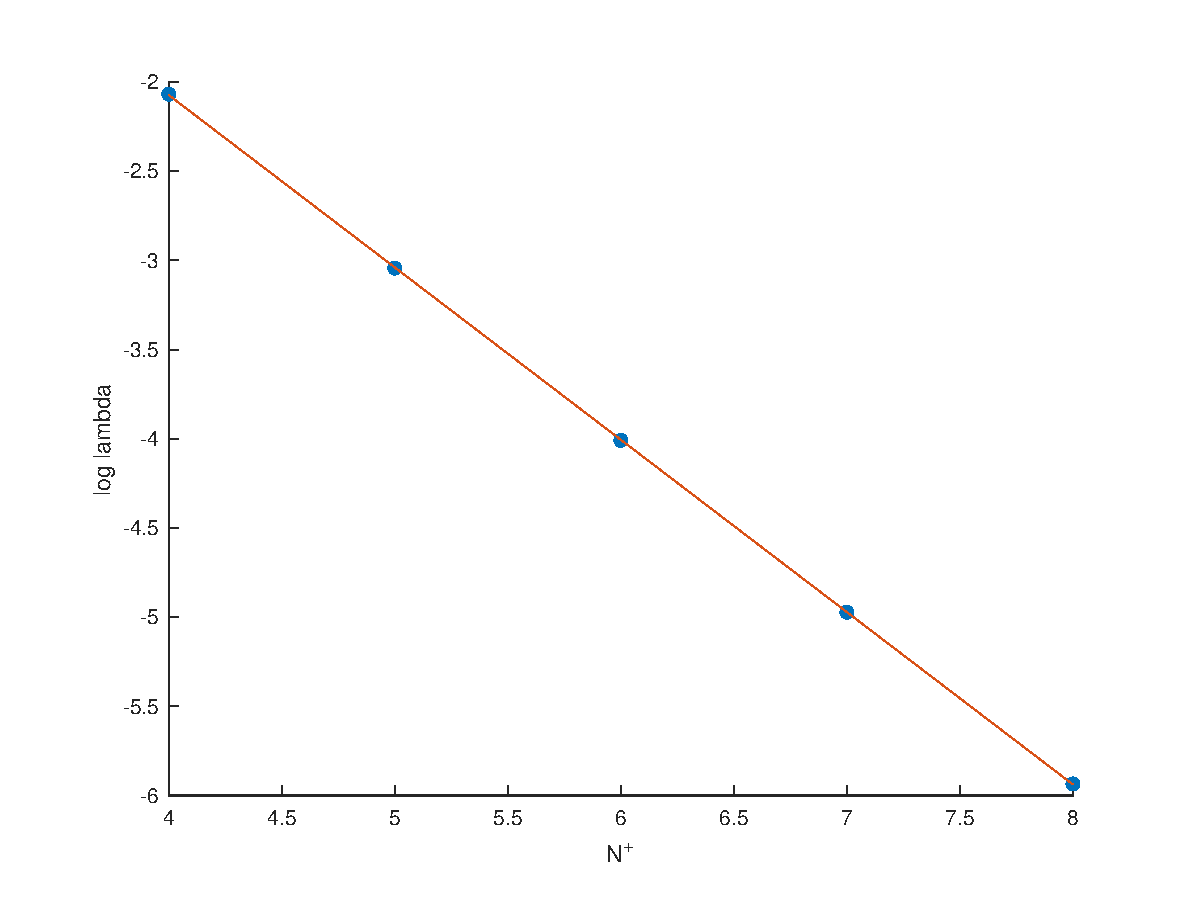
\includegraphics[width=10cm]{dnlslog.eps}
\label{fig:spec1}
\caption{Stable double pulse}
\end{figure}

The slope of best-fit line is $-0.9660$ and $\log r = -0.9206$; the error is about $0.05$, which is great!

\end{document}